\section{Result and discussion}
The YOLO-NAS has YOLO-NAS-L, YOLO-NAS-M, and YOLO-NAS-S variants as we have discussed earlier and the result and discussion are tailored to individual performance characteristics of each model, and every model has three paths to choose from; the best model, average model and latest model, and particularly  the inference performed after the training were used best path of each model.
\subsection{Dataset and Preprocessing}
In section [\nameref{datset}] I have discussed the dataset properties
\begin{figure}[H]
    \centering
    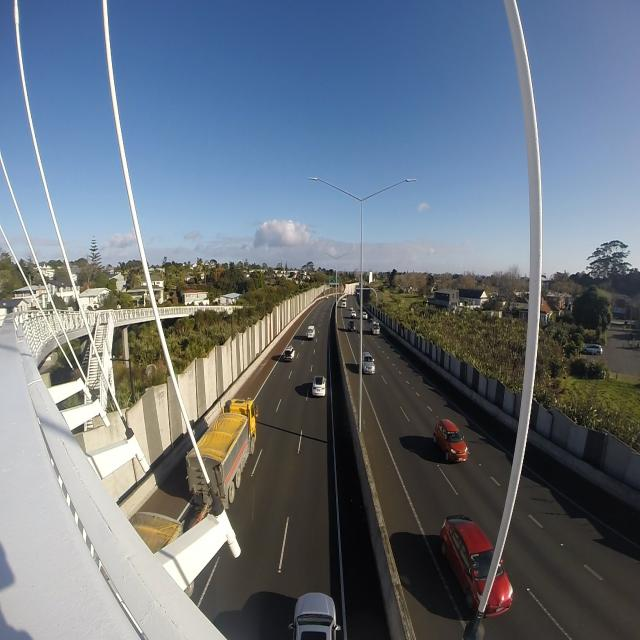
\includegraphics[width=\linewidth]{tex/img/sample_dataset.jpg}
    \caption{sample image for all model}
    \label{fig:sample_dataset}
\end{figure}
%%%%%%%%%%%%%%%%%%%%%%%%%%%%%
%YOLO_NAS_S
%%%%%%%%%%%%%%%%%%%
\begin{figure}[H]
  \begin{minipage}{0.48\textwidth}
    \centering
    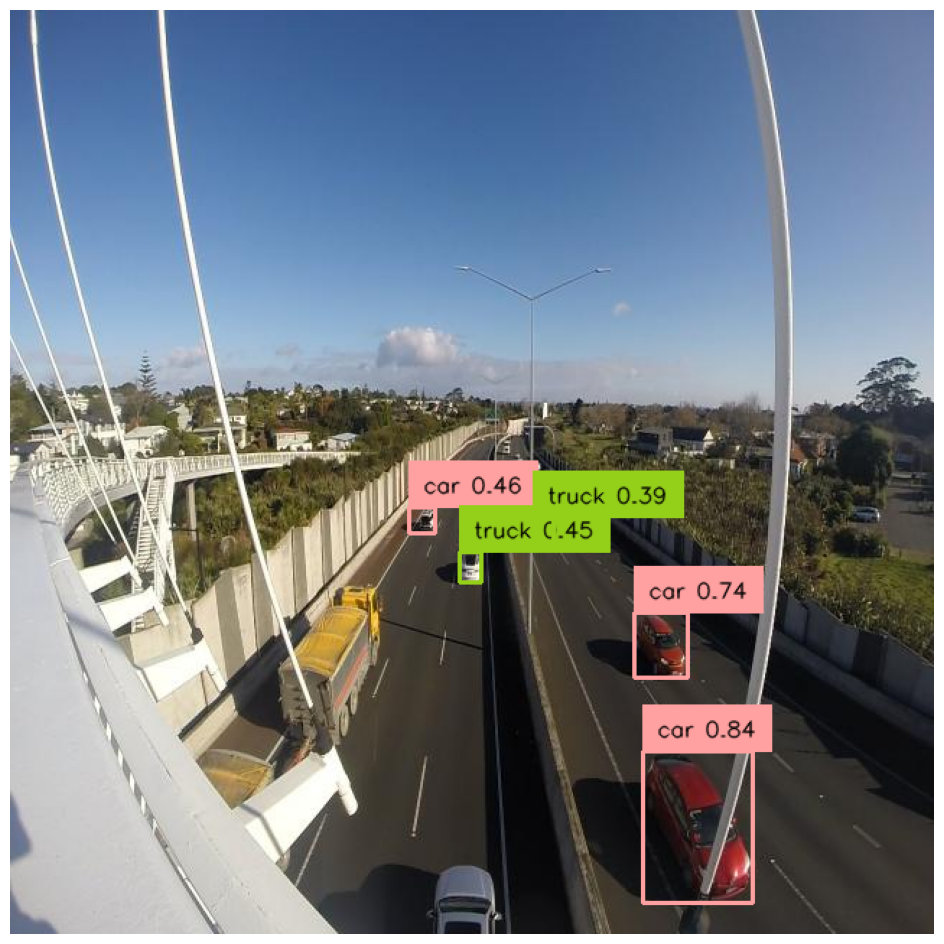
\includegraphics[width=\linewidth]{tex/img/S-before_trainingYN_S.png}
    \caption{YOLO-NAS-S: Inference 
    on the Model before training}
    \label{fig:YOLO-NASSM_vs_other_models}
  \end{minipage}%
  \begin{minipage}{0.5\textwidth}
    \centering
    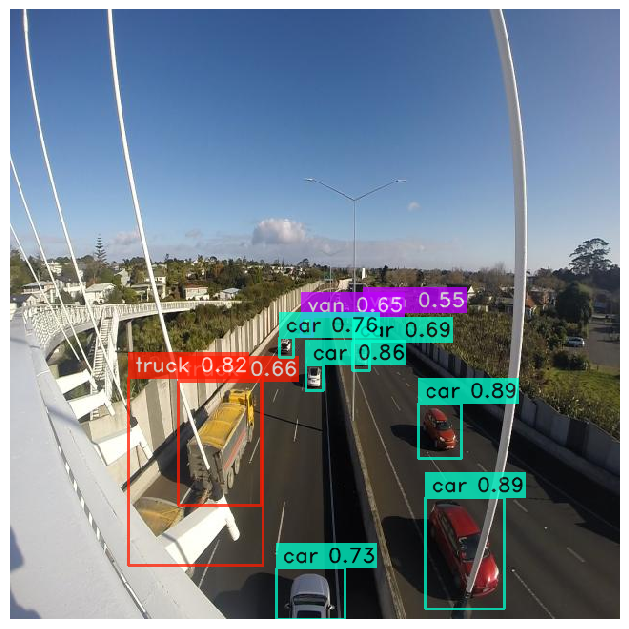
\includegraphics[width=\linewidth]{tex/img/S-After training_YN_S.png}
    \caption{YOLO-NAS-S: Inference on the Model after training}
    \label{fig:YOLO-NAS_vs_other_models}
  \end{minipage}
  \caption{YOLO-NAS: Inference on the model before and  after training .}
\end{figure}

\begin{figure}[H]
    \centering
    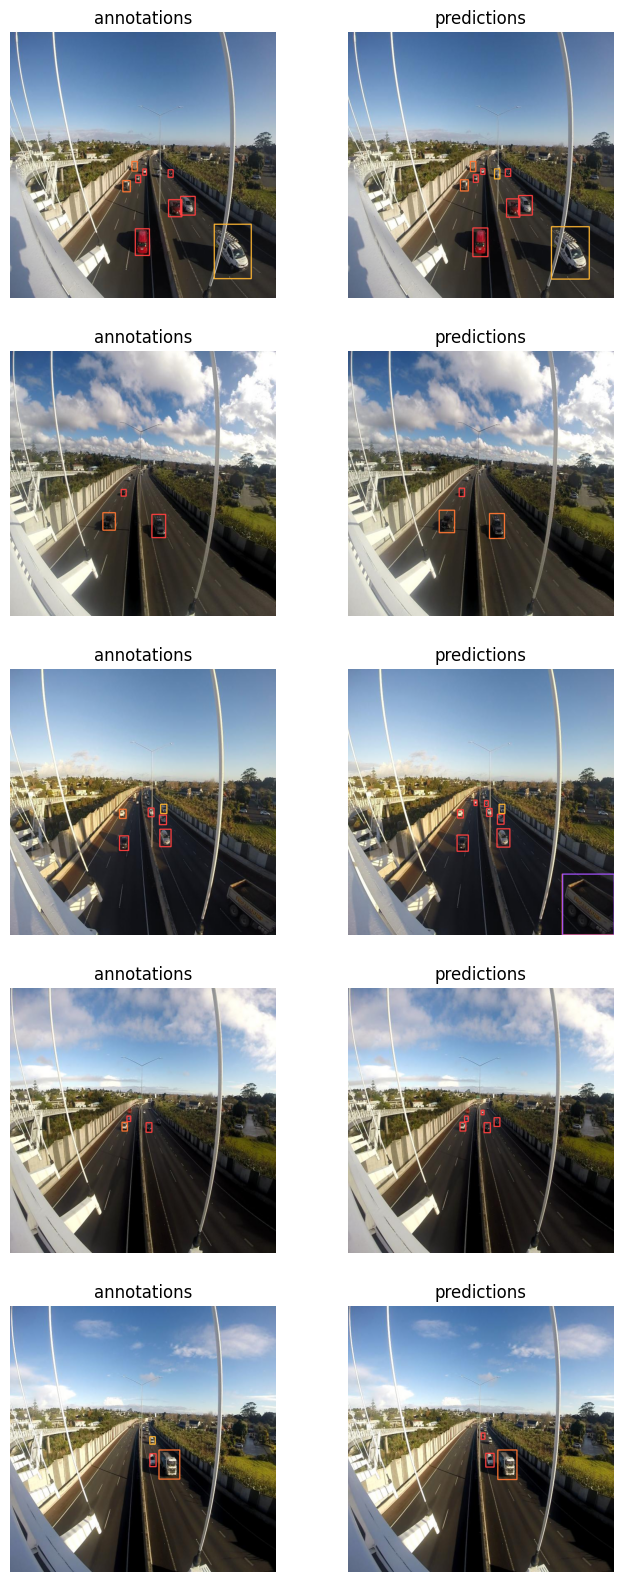
\includegraphics[width=0.6\linewidth]{tex/img/S-annotation_&_prediction.png}
    \caption{Annotation and Prediction}
    \label{fig:L-annot-pred}
\end{figure}

\begin{figure}[H]
    \centering
    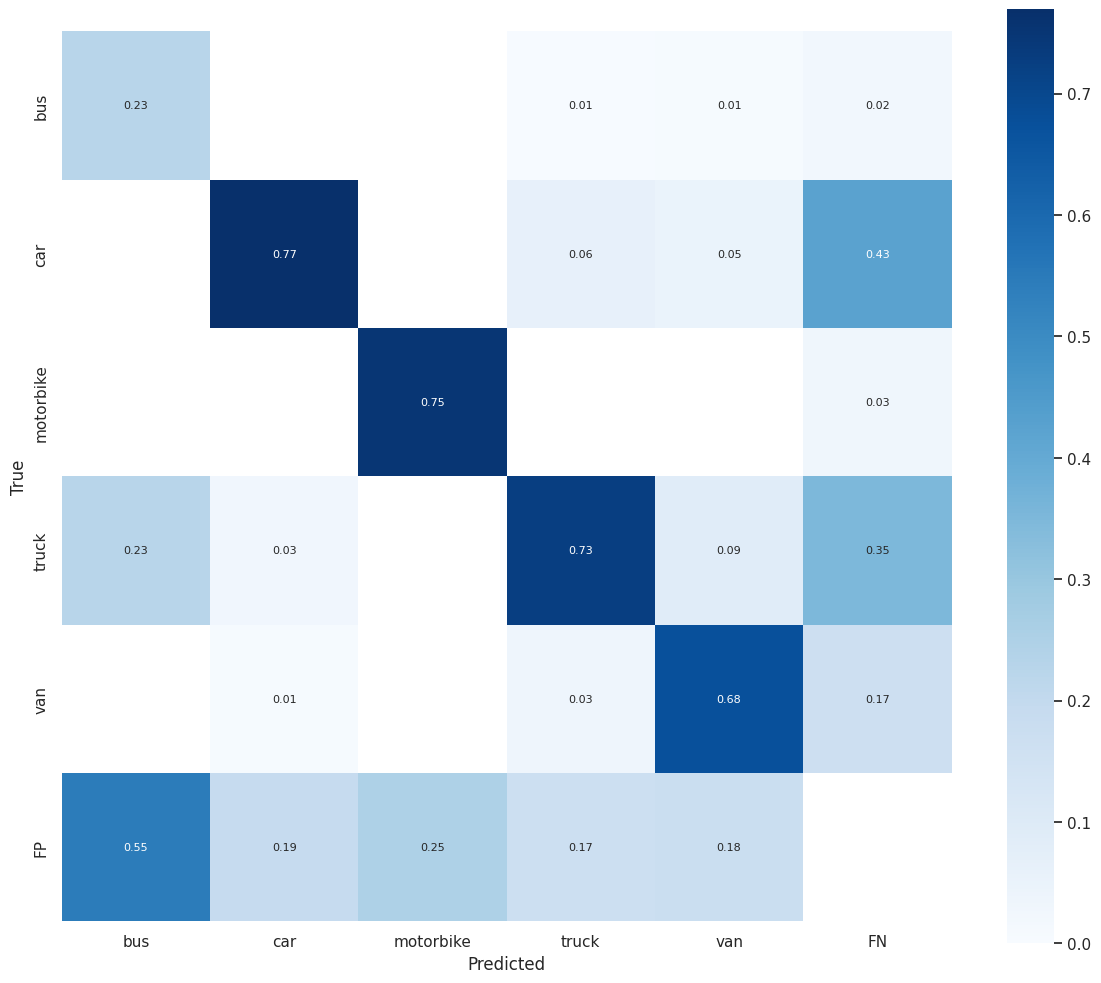
\includegraphics[width=\linewidth]{tex/img/S-Overall_or_confusionMatrix.png}
    \caption{YOLO-NAS-S Overall results }
    \label{fig:ConfusionMatrixY-N-S}
\end{figure}
%%%%%%%%%%%%%%%%%%%%%%%%
%YOLONAS-M
%%%%%%%%%%%%%%%%%%%%
\begin{figure}[H]
  \begin{minipage}{0.48\textwidth}
    \centering
    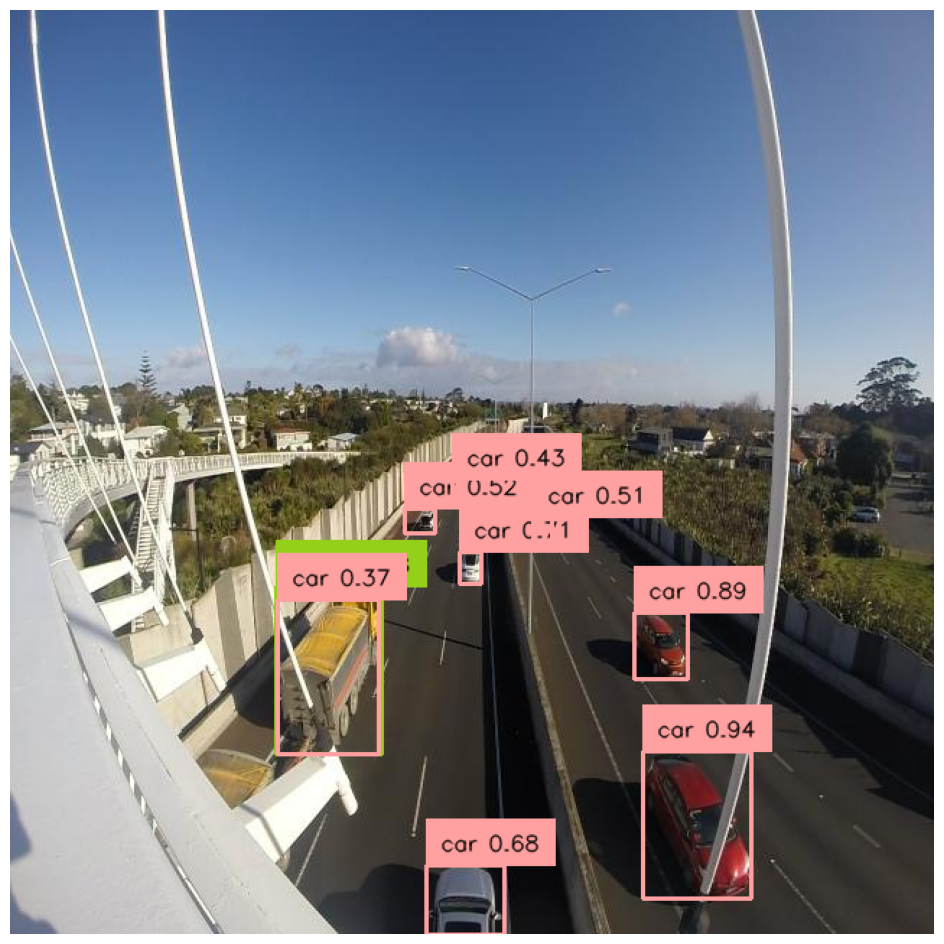
\includegraphics[width=\linewidth]{tex/img/M-before_training.png}
    \caption{YOLO-NAS-M: Inference 
    on the Model before training}
    \label{fig:YOLO-NASSM_vs_other_models}
  \end{minipage}%
  \begin{minipage}{0.5\textwidth}
    \centering
    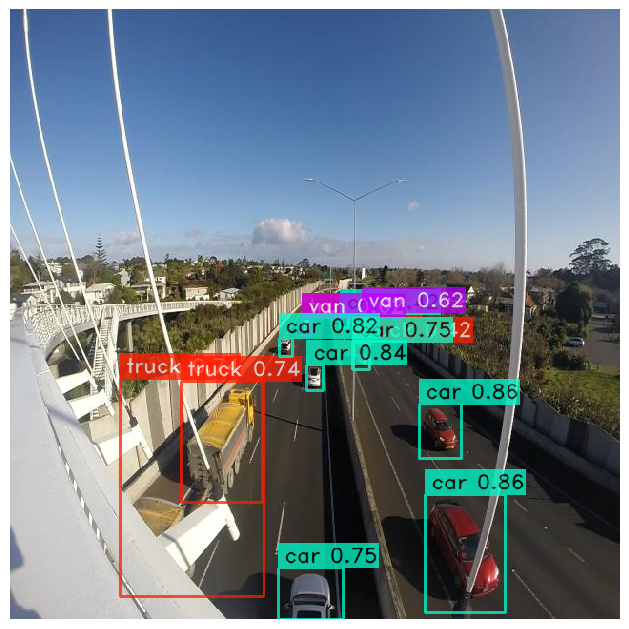
\includegraphics[width=\linewidth]{tex/img/M-after training.png}
    \caption{YOLO-NAS-M: Inference on the Model after training}
    \label{fig:YOLO-NAS_vs_other_models}
  \end{minipage}
  \caption{YOLO-NAS-M: Inference on the model before and  after training .}
\end{figure}

\begin{figure}[H]
    \centering
    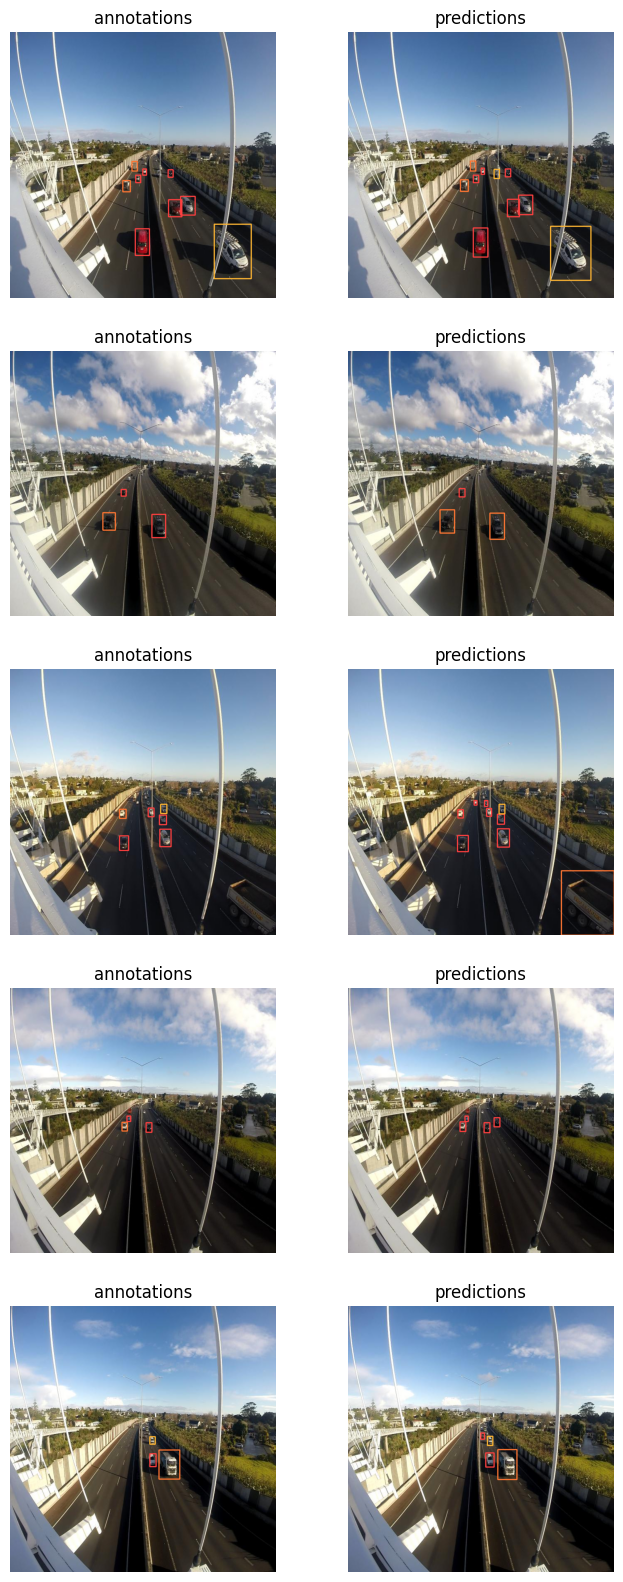
\includegraphics[width=0.6\linewidth]{tex/img/M-Annotation_&_Predictions.png}
    \caption{Annotation and Prediction}
    \label{fig:L-annot-pred}
\end{figure}

\begin{figure}[H]
    \centering
    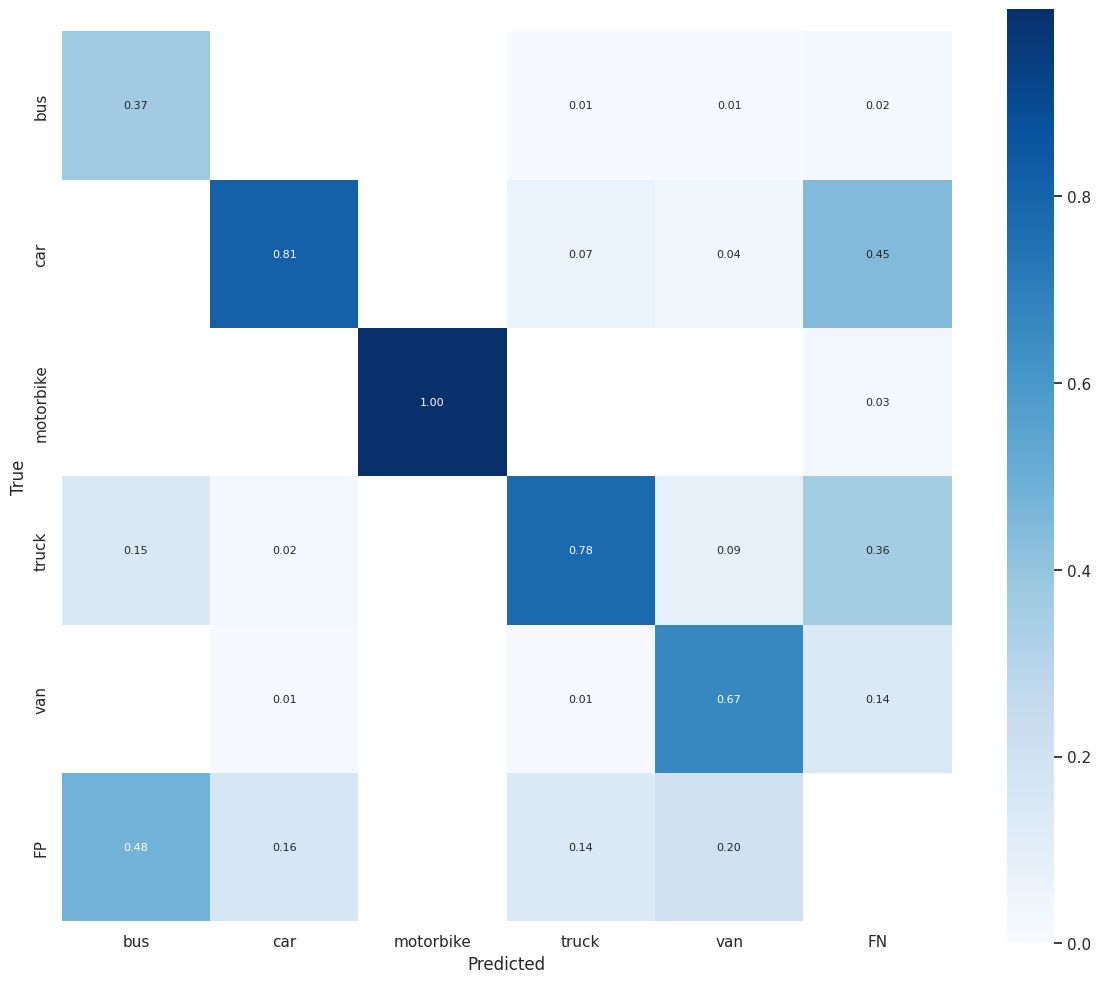
\includegraphics[width=\linewidth]{tex/img/M-confiusion.png}
    \caption{YOLO-NAS-M Overall results }
    \label{fig:ConfusionMatrixY-N-S}
\end{figure}

%%%%%%%%%%%%%%%%%%%%%%%%%%%%%%
%YOLO-NAS-L
%%%%%%%%%%%%%%%%%%%%%%%%%%
\begin{figure}[H]
  \begin{minipage}{0.48\textwidth}
    \centering
    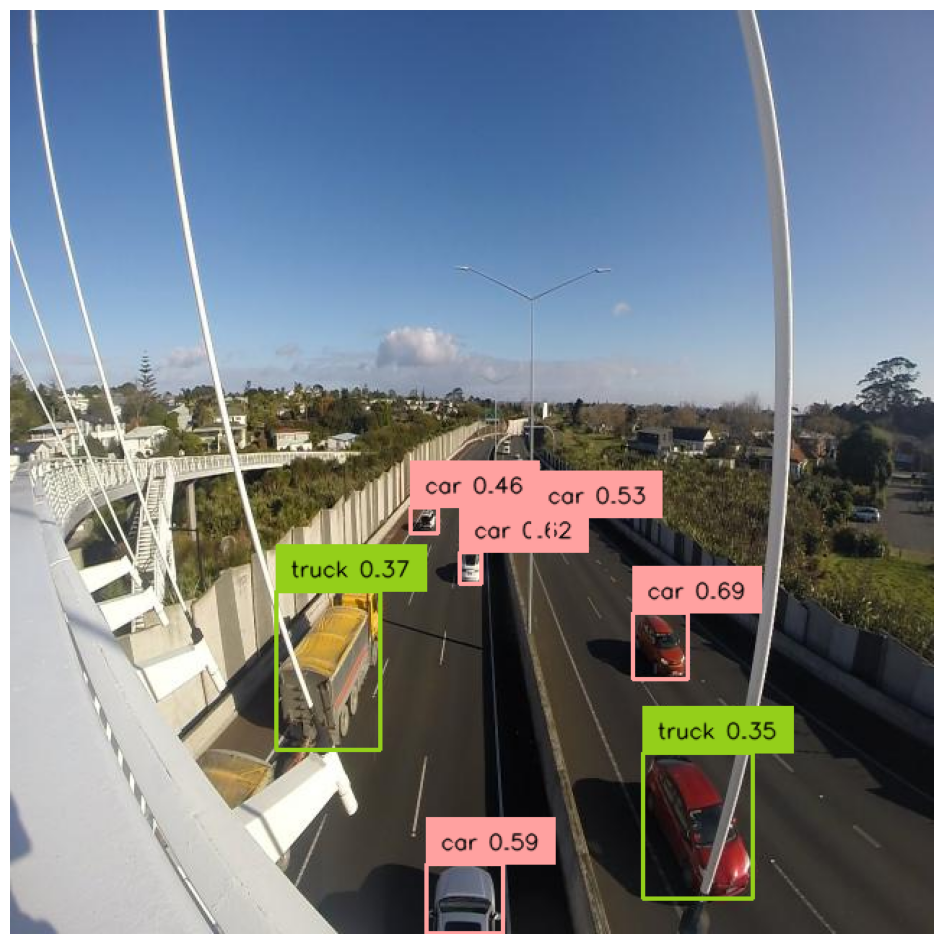
\includegraphics[width=\linewidth]{tex/img/L-before_training.png}
    \caption{YOLO-NAS-L: Inference 
    on the Model before training}
    \label{fig:YOLO-NASSL_vs_other_models}
  \end{minipage}%
  \begin{minipage}{0.5\textwidth}
    \centering
    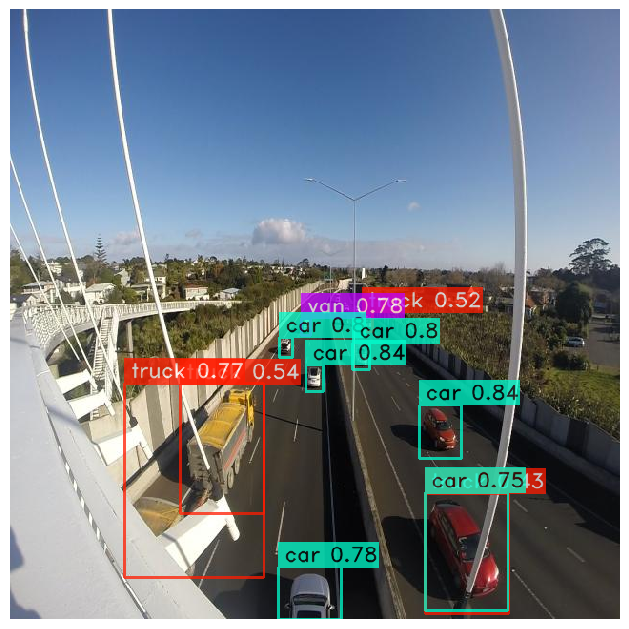
\includegraphics[width=\linewidth]{tex/img/L-after_training.png}
    \caption{YOLO-NAS-L: Inference on the Model after training}
    \label{fig:YOLO-NAS_vs_other_models}
  \end{minipage}
  \caption{YOLO-NAS-L: Inference on the model before and  after training .}
\end{figure}


\begin{figure}[H]
    \centering
    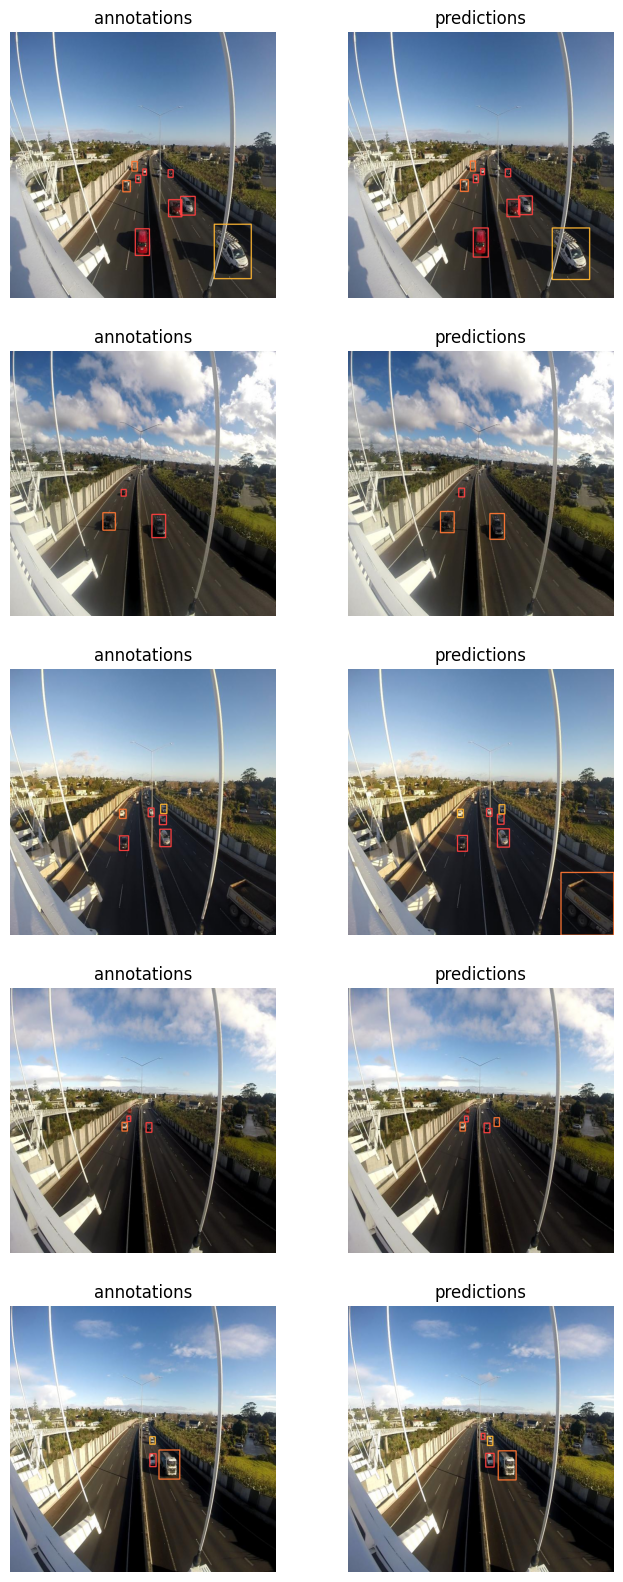
\includegraphics[width=0.6\linewidth]{tex/img/L-annotations_predictions.png}
    \caption{Annotation and Prediction}
    \label{fig:L-annot-pred}
\end{figure}

\begin{figure}[H]
    \centering
    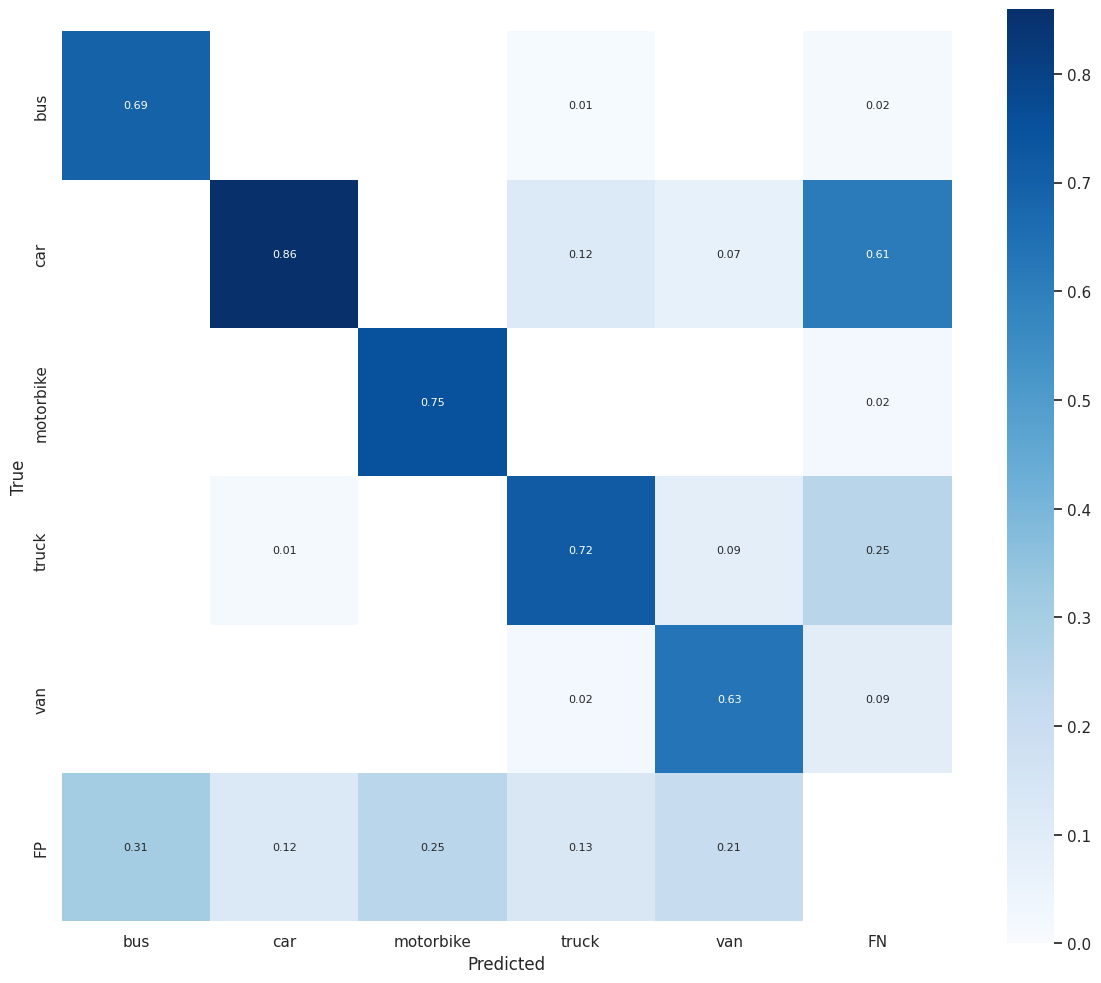
\includegraphics[width=\linewidth]{tex/img/L-confusion_matrix.png}
    \caption{YOLO-NAS-L Overall results }
    \label{fig:ConfusionMatrixY-N-S}
\end{figure}
\subsection{Training and Implementation Details}
For all of the models, I’ve used a batch size of 16, and trained for 20 epochs using NVIDIA Tesla T4 GPU. I implemented and trained the models using Google Colab. 

I have tweaked various hyperparameters for this work. I have set the ”average best models” to true, warm-up models linear epoch step, initial learning rate for warm-up as 1e-6, learning rate decay factor during warmup epochs as 3, initial learning rate as 5e-4, learning rate decay mode as cosine, cosine-final learning rate ratio as 0.1, optimizer as Adam, weight decay in optimizer parameters as 0.0001. I have used zero weight decay on bias and batch-normalization and leveraged exponential moving averaging with a decay factor of 0.9 and decay type as a threshold with the” mixed precision” set to true.
\newpage
\subsection{Analysis of Performance for YOLO-NAS}

\begin{table}[!htbp]
    \centering
    \caption{Analysis of Performance for YOLO-NAS}
    \label{tab:my_label}
    \footnotesize
    \begin{tabular}{|c|c|c|c|c|c|c|c|c|}
    \hline
     Models &  Loss\_cls&  Loss\_iou& Loss\_dfl & Loss &  Precision@0.5&  Recall@0.5&  mAP@0.5& F1@0.5\\
    \hline
    NAS-Small&  0.682&  0.1709&  0.7117&  1.465&  0.07896&  0.8864&  0.6792& 0.14077\\
    \hline
    NAS-Medium& 0.67099 &  0.1688&  0.7356&  1.4609& 0.0917 &  0.9114 & 0.7007 & 0.1596\\
    \hline
    NAS-Large& 0.6535 &  0.1617&  0.7189& 1.4172 &  0.11563&  0.9116&  0.7269& 0.19652\\
         \hline
    \end{tabular}
\end{table}
YOLO-NAS has three models: Large, Medium, and Small.The model with the highest precision NAS-S, achieving a precision of 78.8\%.The model with the highest recall, mAP, and F1 is NAS-M, achieving a recall of62.7\%, a mAP@0.5of69.8\%, and an F1@0.5of67.85\%.Full results, including the losses calculated from the different loss functions, can be found in table \ref{tab:my_label}

